\section{Разработка главной страницы сайта}
\label{sec:practice}

Главная страница сайта состоит из нескольких отдельных компонент:
\begin{itemize}
	\item навигационная панель;
	\item блок с отрывком из введения с кнопкой <<читать далее>>;
	\item блок с общим описанием диалома и его уникальности;
	\item блок с примерами пользовательского интерфейса;
	\item таблица со списком использовавшихся источников.
\end{itemize}

Помимо того, страница, как и большинство других \gls{html}-страниц, разбита на блоки \lstinline[language=HTML]{<head>} и \lstinline[language=HTML]{<body>}, служащие для описания метаинформации и разметки содержимого соотстветвенно.

\begin{figure}[h]
  \centering
    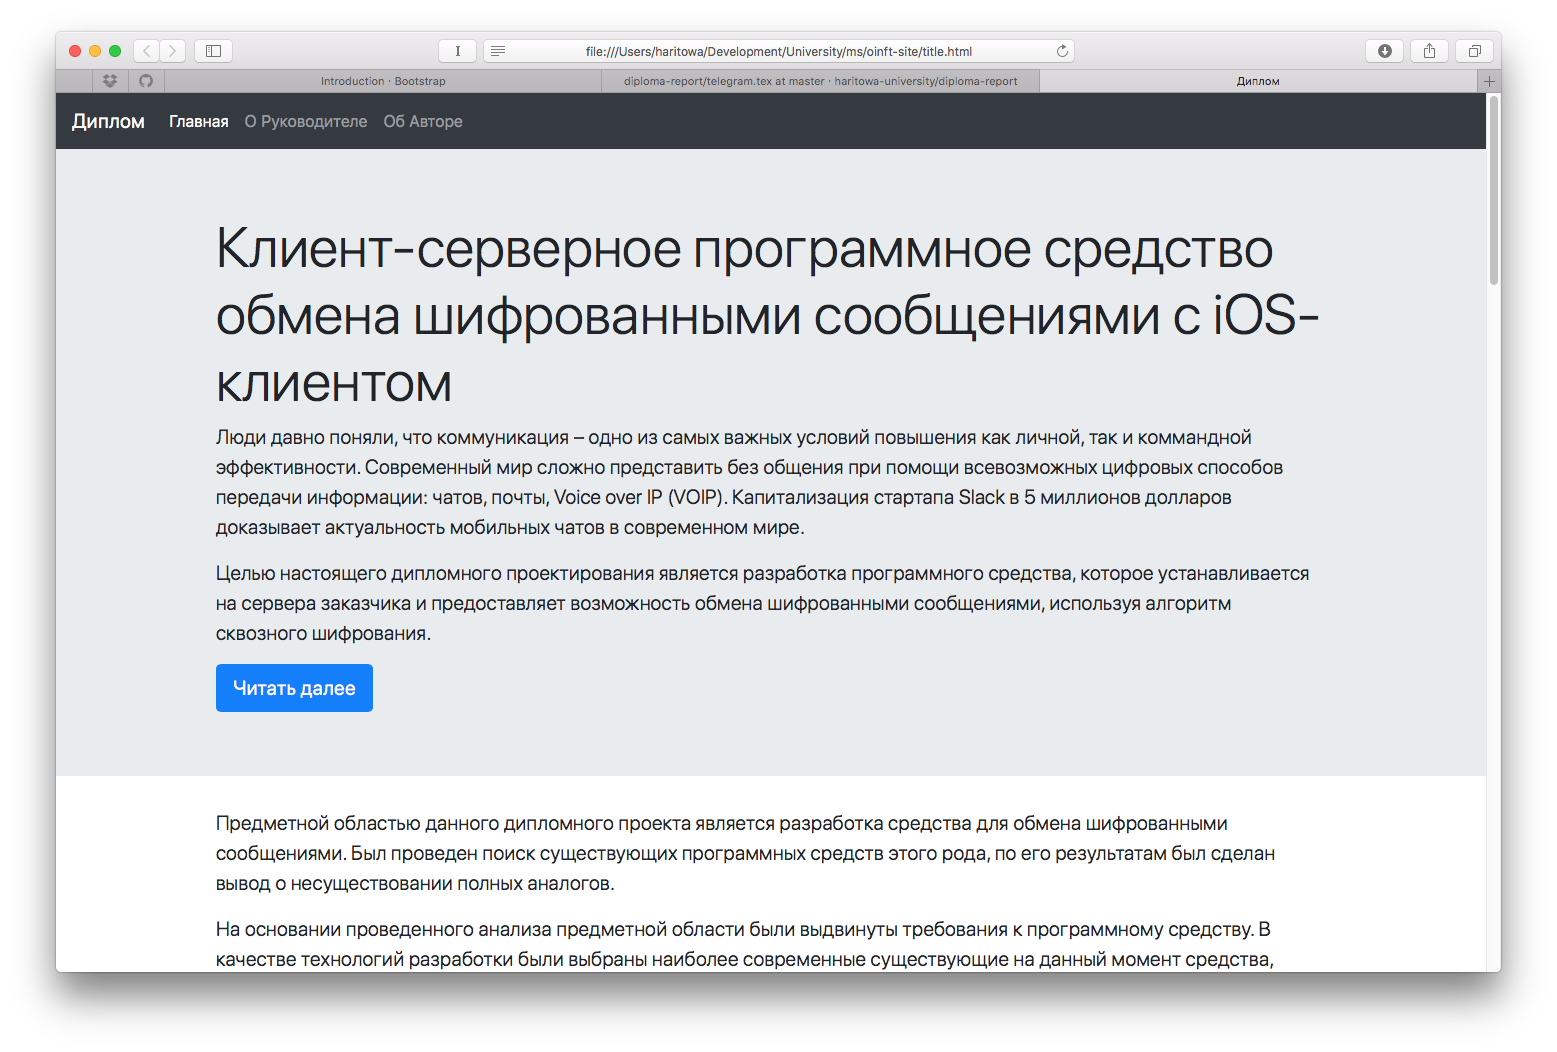
\includegraphics[width=0.8\textwidth]{inc/img/title}
  \caption{Схема общения при помощи MTProto}
  \label{sec:analysis:research:analogs:telegram:mtproto1}
\end{figure}